% %%%%%%%%%%%%%%%%%%%%%%%%%%%%%%%%%%%%%%%%%%%%%%%%%%%%%%%%%%%%%%%%%%%%%%%%%%%%%
% %%%%%%%%%%%%%%%%%%%%%%%%%%%%%%%%%%%%%%%%%%%%% Simulations of Giant Pulsations
% %%%%%%%%%%%%%%%%%%%%%%%%%%%%%%%%%%%%%%%%%%%%%%%%%%%%%%%%%%%%%%%%%%%%%%%%%%%%%

\chapter{Evolution of Giant Pulsations}
\label{ch_pgs}



% =============================================================================
% =============================================================================
% =============================================================================
\section{Drifting Ground Signatures}

In this model, azimuthal offset is indicated by complex phase per $\exp \arg{i \azm \phi}$. 

For the most part, each field exhibits a uniform phase. Poloidal electric and magnetic fields are overwhelmingly real. Toroidal electric and magnetic fields are overwhelmingly imaginary. 

\todo{Get typical phase ranges. }

The north-south component of the magnetic ground signatures is uniformly imaginary. By comparing to \cref{fig_BqE_J_1} it's clear that the ostensibly real regions in \cref{fig_BqE_phase_J_1} are an illusion; they coincide with near-zero field magnitudes. 

Note that in \cref{fig_BqE_phase_J_1,fig_BfE_phase_J_1}, phase is defined as: $\, \arctan \left| \frac{ \mathbb{I}\mathrm{m} \, B }{ \mathbb{R}\mathrm{e} \, B } \right|$. 

\begin{figure}[H]
    \centering
    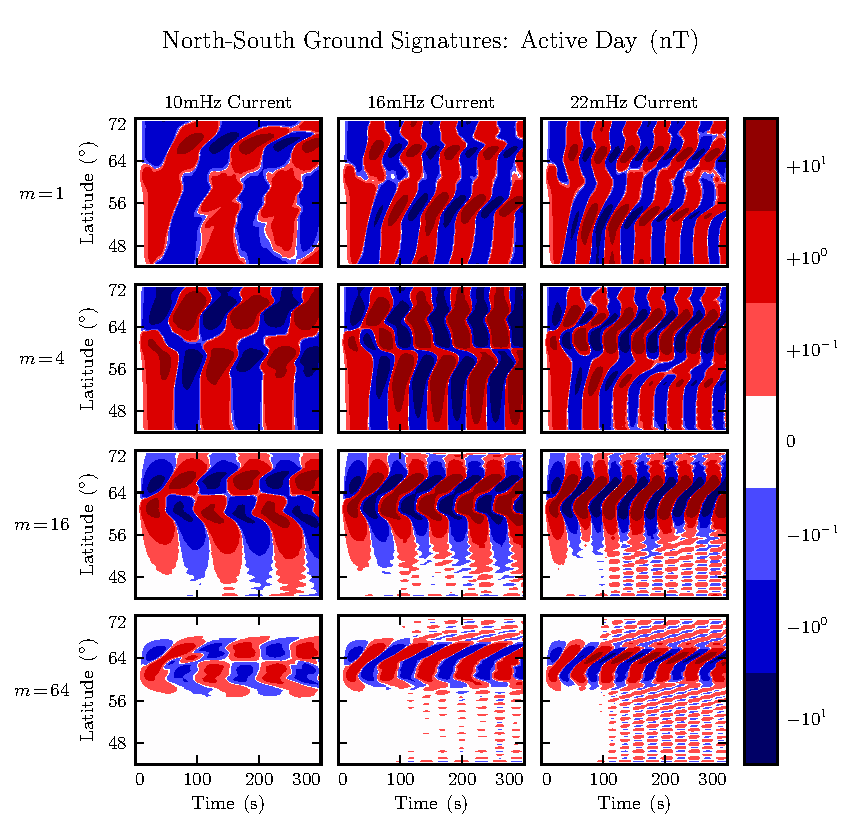
\includegraphics[width=\textwidth]{figures/BqE_J_1.pdf}
    \caption[North-South Ground Signatures: Active Day]{}
    \label{fig_BqE_J_1}
\end{figure}

\begin{figure}[H]
    \centering
    \includegraphics[width=\textwidth]{figures/BqE_phase_J_1.pdf}
    \caption[North-South Ground Signature Phases: Active Day]{}
    \label{fig_BqE_phase_J_1}
\end{figure}

In contrast, the phase of the east-west aligned magnetic field evolves visibly over the course of an oscillation. This is particularly evident in the third row, $m=16$. The effect is present at latitudes where the field intensity is high (though not the highest). 

The near-peak-amplitude phase rotation for \SI{100}{\mHz} driving at $m=16$ can be eyeballed around $\frac{\pi}{8}$ in half a wave period (\SI{50}{\second}). This corresponds to $\sim$ \SI{0.3}{\deg/\second}. This is within an order of magnitude of Glassmeier's\cite{glassmeier_1999} much-cited event, which had a horizontal phase speed of $\SI{0.135}{\degree/\second}$. 

\begin{figure}[H]
    \centering
    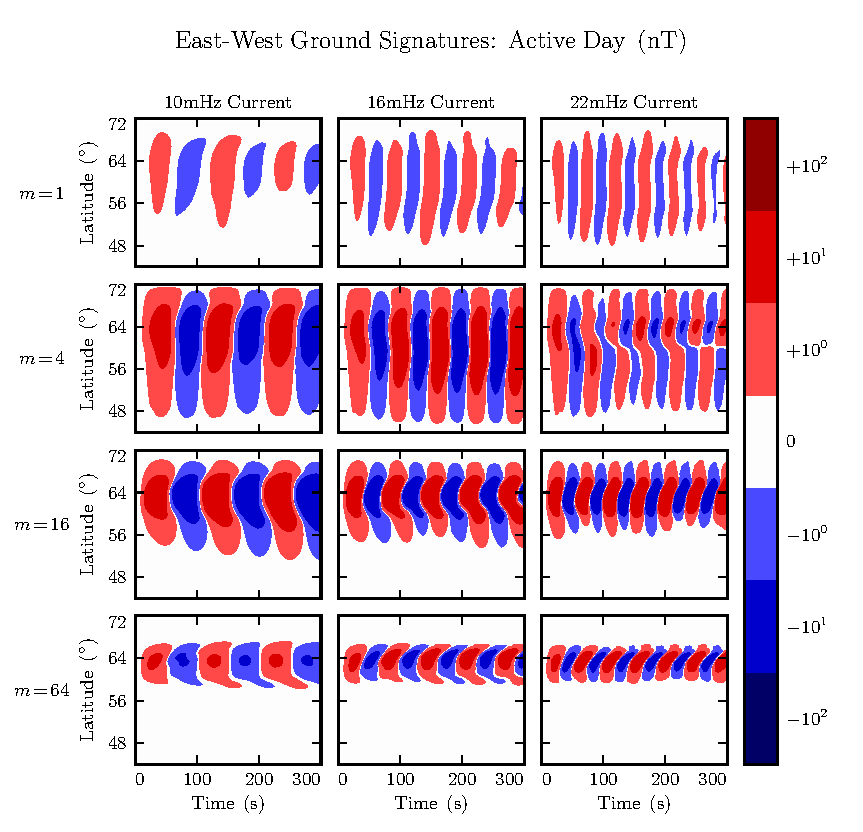
\includegraphics[width=\textwidth]{figures/BfE_J_1.pdf}
    \caption[East-West Ground Signatures: Active Day]{}
    \label{fig_BfE_J_1}
\end{figure}

\begin{figure}[H]
    \centering
    \includegraphics[width=\textwidth]{figures/BfE_phase_J_1.pdf}
    \caption[East-West Ground Signature Phases: Active Day]{}
    \label{fig_BfE_phase_J_1}
\end{figure}









